% !TeX root = ./mSys_MAIN_rev2.tex
One of the highlights of this study is that is shows, independently of its condition, that microbiota follows Taylor’s law. We have seen that in each case the value of the scaling index is always less than the unity (using standard deviation as the dispersion measurement), which provides us with information about the community structure. This means that, in relative terms, the most abundant elements in the population are less volatile to perturbations than the less abundant ones. The explanation for this universal pattern is not clear although some hypotheses have been tested in other studies, such as the presence of negative interactions in the population \cite{kilpatrick}, and a demonstration that this may depend on reproductive correlation \cite{ballantyne}. Nevertheless, none of these explanations are sufficient when it comes to microbiota, as the term reproduction is diffuse the interactions between its components are not only based on competition \cite{joao, mehta, bucci}. Moreover, even such negative interaction may not effectively yield values less than the unity when referring to a bacterial species (41). Nonetheless, the values obtained in all cases were very similar to each other, which may suggest that the community structure is preserved throughout the different scenarios studied herein.

The second parameter provides information about noise and can be directly linked to the variability or fluctuation amplitude of the population over time. It is a direct estimator of the stability of the system under study. As we have shown above, the healthy subset of each study has lower variability than the non-healthy subset, when dealing with adult subjects. Interestingly, the variability parameter was higher in the healthy subset in the study of discordant twins suffering from kwashiorkor disease \cite{kwashiorkor}. In this respect, research has shown that infant microbiota needs to develop toward a definite, adult state \cite{koenig}. This implies that temporal variability is greater in children than in a healthy adult, which should be temporally stable. Thus, our results could indicate this variability is necessary in order to reach that adult state. Furthermore, as we wanted to see how this variability shifted over time, we calculated the changes in this parameter for the samples which had enough time sampling. As shown in Figure \ref{fig:tempevo1}, the variability of microbiota fluctuated over time. Interestingly, Figure \ref{fig:tempevo2} shows how this parameter reflected the two antibiotic intakes in one of the patients in the study by Dethlefsen and Relman \cite{antibiotic} particularly the apparent resilience of the microbiota due to the reduced increase in variability during the second antibiotic intake.

The primary hypothesis of this work is that, in adults, having a healthy microbiota means that the microbial population is stable over time.  This stability means the microbiota does not shift and become susceptible to external or internal perturbations causing dysbiosis. In order to use the valuable information provided by the empirical law of Taylor’s work, herein we have proposed the use of Langevin’s equation to model how stability ranking changed  over time. While the system noise component can be directly measured as its variability, the other main term needs to be inferred from the model. This term, which we have named "fitness", enables the system to remain stable when confronted with potential perturbations. In ecological terms, this could represent the nature of interactions present among bacteria, between bacteria and other minority populations, such as fungi or archaea, between bacteria and the viral component in microbiota, and interactions between the host and the whole microbiota. As this is a first step to model the temporal stability of microbiota, and given its complex nature, we calculated fitness using the Fluctuation Dissipation Theorem as a first approximation \cite{FD}. Thus, future works are required to model the fitness of microbiota in order to provide a more accurate model with higher predictive power. 

By solving Langevin’s differential equation, we obtain a phase diagram where each microbiota sample can be placed by its fitness and variability into one of two phases, according to the stability ranking of the system. As shown by the phase--space in Figure \ref{fig:main3}, three different conditions can occur. The first is a healthy microbiota with some fluctuations, as shown by one of the subjects in Caporaso \emph{et al.}'s study \cite{moving}. Because this case would have good fitness, its temporal variability would not place the microbiota in the unstable phase of the diagram. Secondly, we have a subject from the study by Dethlefsen and Relman \cite{antibiotic} whose microbiota was perturbed twice by an antibiotic intake, undergoing sufficient change so as to lose its stability, and hence be placed in the unstable part. In this location, it is more sensitive to potential perturbations such as, for example, opportunistic infections. In the third and last condition, the subject was already in the unstable phase due to a health issue, i.e. IBS. This can be observed in one of the patients in Durban \emph{et al.} \cite{IBS}. In addition, it was shown that this subject’s health status improved during the experiment, implying that his/her microbiota also recovered stability. Interestingly, in the study made by David \emph{et al.} \cite{hostlife} the subject who had a Salmonella infection during the experiment underwent a significant shift in variability with eventual recovery from the perturbed state (see Supplementary Figure S\ref{supfig:HLS_xWSummary}).

\begin{supfig}
	\centering
	%\vspace*{-10mm} % Corrects overbox of the figures
	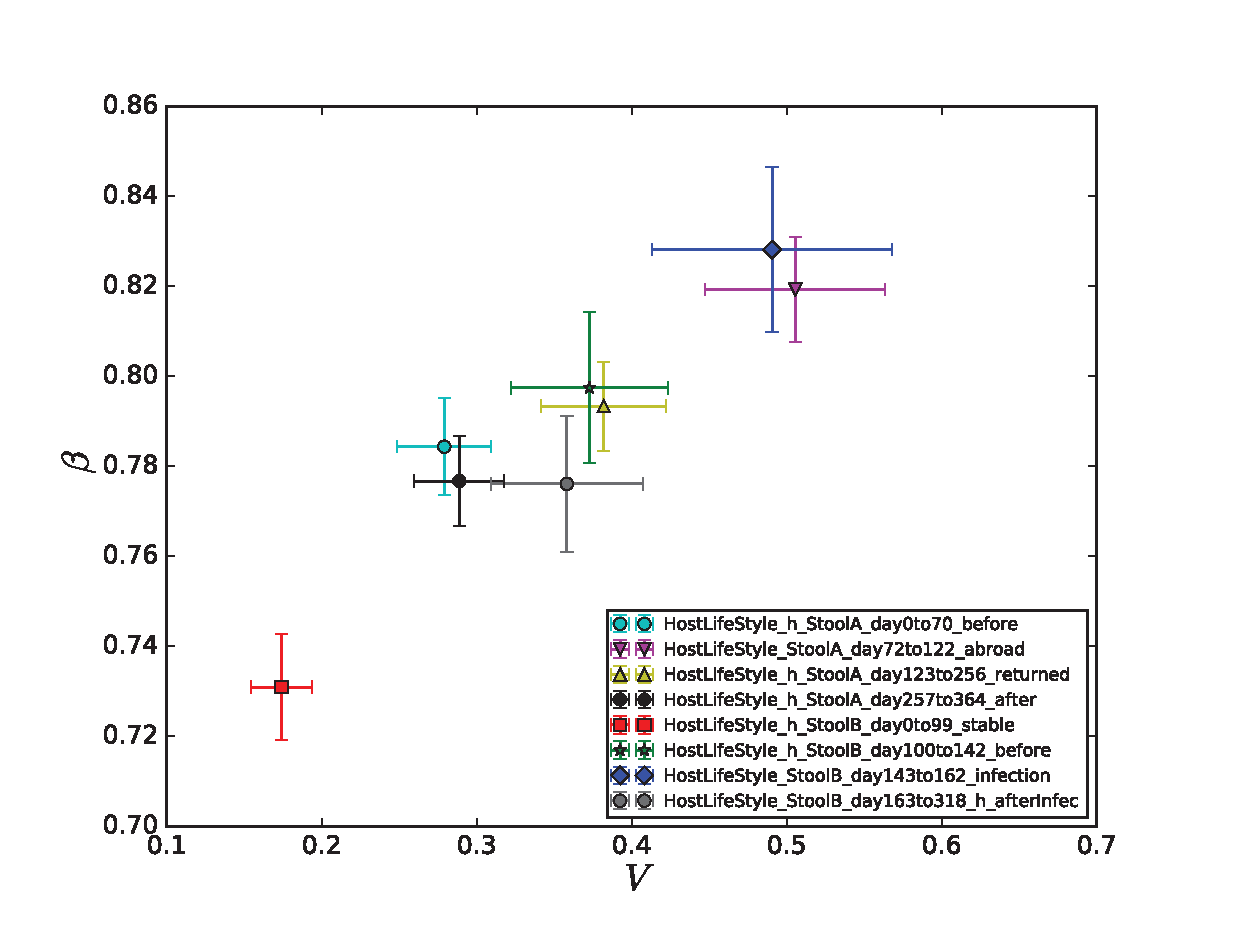
\includegraphics[width=0.99\textwidth]{figs/supfig_HLS_xWSummary.eps}
	\caption{Taylor's law parameter space for intervals concerning gut microbiota in the host lifestyle study\cite{hostlife}. We observe that subject \emph{B}, who suffered a Salmonella infection during the experiment, had a relevant shift in the parameters from \emph{\_before} to \emph{\_infection} and a final recovery from the perturbed state to \emph{\_afterinfec}, which lies in the parameter area compatible with the healthy and stable intervals (see Supplementary Table S\ref{tab:Ab-IBS-HLS}). Subject \emph{A} also had a shift in variability from \emph{\_before} to \emph{\_abroad} and back to \emph{\_returned}, also in the proximity zone of healthy and stable periods.}
	\label{supfig:HLS_xWSummary}
\end{supfig}
 
Specifically, in the host lifestyle study \cite{hostlife}, the presence of \emph{rank stability islands} among medium--ranked taxa is an interesting feature revealed by the analysis of rank stability at different time periods in subject \emph{A}. Interestingly, this stability was compromised when the period was not an ordinary one, suggesting that those taxa were sensitive to changes in lifestyle. Among the genera identified as \emph{rank stability islands}, \emph{Lachnobacterium} and \emph{Clostridium} were catalogued as genera predictive of dysbiosis in the work of Larsen and Dai \cite{rsi_dysbiosis}, which analysed the same dataset \cite{hostlife}. Furthermore, research has recently confirmed a clear relationship between \emph{Actinomyces} and conventional adenoma \cite{rsi_actino}, one of the two main precursors of the colorectal cancer. Finally, \emph{Eggerthella} is an opportunistic pathogen that is often associated with serious gastrointestinal pathology \cite{rsi_egg}.

One might  question the role of these taxa as key players in the phase transition of the microbiota and wonder whether they are more susceptible to perturbations than the most abundant taxa. The types of interactions that could sustain this particular behavior are unclear, as these non-abundant taxa are usually excluded from dynamic studies to obtain a community matrix. Further experiments and data analysis are needed to clarify whether \emph{rank stability islands} are a widespread feature of microbiotas and whether they appear at lower taxonomic levels too.

Notwithstanding the above, we should be aware that the above hypothesis is too simplistic to directly apply to reality. Indeed, the situation is more complex than the idea that healthy people can be distinguished from non-healthy people in solely compositional terms, as highlighted by Moya and Ferrer in their recent review \cite{Moya_trends}. There are several feasible scenarios in which we can consider microbiota to be stable, irrespective of its compositional shifts over time. For example, it may depend on the ability of the microbiota to recover its initial composition (resilience), or its ability to recover its original function despite its composition (functional redundancy). What we have shown in this work could be explained as the transition of stable microbiota into a state of dysbiosis.  

This is a first step towards understanding microbiota stability, although the model presents some limitations and thus further research is required. From a biological perspective, many questions arise from this work. We have observed the same pattern in Taylor’s parameters under all the conditions studied, but a pertinent question is whether this is really a universal feature in the hugely diverse microbial niches. Furthermore, another relevant question relates to mechanisms involved in maintaining the population structure.  Undoubtedly, the nature of the interactions between community components has a great bearing on this issue, and this is related to community fitness, as mentioned above. How we should address community fitness remains unclear, but studies like the one by Tikhonov  \cite{tikhonov} could point us in the right direction and help us to unravel the complexity of microbiota and its relationship to host health.